\documentclass[12pt,a4paper,openright,twoside]{book}
\usepackage[utf8]{inputenc}
\usepackage{disi-thesis}
\usepackage{code-lstlistings}
\usepackage{notes}
\usepackage{shortcuts}
\usepackage{acronym}
\usepackage{cleveref}

\acrodef{PC}{Personal Computer}
\acrodef{VNC}{Virtual Network Computing}
\acrodef{RDP}{Remote Desktop Protocol}
\acrodef{TPDU}{Transport Protocol Data Units}
\acrodef{PDU}{Protocol Data Units}
\acrodef{SVC}{Static Virtual Channels}
\acrodef{DCV}{Dynamic Virtual Channels}
\acrodef{LAN}{Local Area Network}
\acrodef{IaaS}{Infrastructure as a Service}
\acrodef{PaaS}{Platform as a Service}
\acrodef{SaaS}{Software as a Service}
\acrodef{GaaS}{Gaming as a Service}
\acrodef{FPS}{First Person Shooter}
\acrodef{SLA}{Service Level Agreement}


\school{\unibo}
\programme{Corso di Laurea Triennale in Ingegneria e Scienze Informatiche}
\title{Evoluzione delle Tecnologie di Desktop Remoto}
\author{Matteo Susca}
\date{\today}
\subject{Reti di Telecomunicazioni}
\supervisor{Prof. Franco Callegati}
\session{III}
\academicyear{2023-2024}

% Definition of acronyms
\acrodef{IoT}{Internet of Thing}
\acrodef{vm}[VM]{Virtual Machine}


\mainlinespacing{1.241} % line spacing in mainmatter, comment to default (1)

\begin{document}

\frontmatter\frontispiece

\begin{abstract}
    Negli ultimi decenni, le tecnologie di desktop remoto hanno acquisito crescente rilevanza, trovando applicazione in diversi ambiti, dallo smart working al cloud gaming. Questa tesi si propone di analizzare l’evoluzione e lo stato attuale delle principali tecnologie di desktop remoto, illustrandone i principali protocolli, le caratteristiche e le gli aspetti innovativi. Le prime tecnologie di accesso remoto come l'X Window System e il protocollo VNC hanno aperto la strada a soluzioni moderne come Parsec, ottimizzate per contesti in cui le latenze sono un fattore critico.
    
    Questi strumenti trovano applicazione in diversi contesti moderni, come il telelavoro e l'assistenza remota, dimostrando come la loro adozione possa migliorare 

    L'applicazione di questi strumenti in contesti moderni come il telelavoro e l'assistenza remota, porta alla luce alcuni innegabili vantaggi, come l'abbattimento dei costi e l'aumento della produttività.
    %TODO IAAS
    Tecnologie di desktop remoto vengono frequentemente utilizzate in combinazione a servizi di cloud computing permettondo l'accesso ad un ambiente desktop completo invece di un terminale o singole applicazioni. Questo approccio unisce i vantaggi di scalabilità di un servizio Infrastructure as a Service (IaaS) e la flessibilità di utilizzo offerta dal desktop remoto.

    Verranno infine illustrate possibili prospettive future e l'influenza che tecnologie emergenti come la realtà aumentata e le reti 5G potrebbero avere sulle tecnologie di desktop remoto.
\end{abstract}
    

\begin{dedication} % this is optional
Dedicato a me stesso,

senza il quale non sarei riuscito

a scrivere questa tesi.
\end{dedication}

%----------------------------------------------------------------------------------------
\tableofcontents   
% \listoffigures     % (optional) comment if empty
% \lstlistoflistings % (optional) comment if empty
%----------------------------------------------------------------------------------------

\mainmatter

%----------------------------------------------------------------------------------------
\chapter{Introduzione}
\label{chap:introduction}

Al giorno d'oggi, è sempre più comune incontrare realtà lavorative che offrono la possibilità di lavorare da remoto.
%
La possibilità di connettersi ad un computer aziendale da qualsiasi dispositivo connesso a internet comporta numerosi e innegabili vantaggi,
come l'accesso diretto alla rete aziendale,
l'utilizzo di hardware specifico per alcune attività senza doverlo trasportare fisicamente,
e la flessibilità di lavorare da casa o in mobilità.
%
Tutto questo è reso possibile dalle tecnologie di desktop remoto, che permettono di controllare un computer da un altro dispositivo, ovunque esso si trovi, come se ci si trovasse fisicamente davanti ad esso.

Anche nell'industria videoludica le tecnologie di desktop remoto ricoprono un ruolo importante.
%
Il cloud gaming,
ad esempio, è un servizio che permette di giocare a videogiochi in streaming,
sfruttando la potenza di calcolo di un server remoto.
%
Il colosso tecnologico NVIDIA,
uno dei principali attori in questo settore,
ha dimostrato fin dal 2013 con il servizio NVIDIA GRID di essere in grado di offrire un'esperienza di gioco fluida e di alta qualità,
grazie all'utilizzo di tecnologie di desktop remoto.
%
Ora il servizio è stato ribattezzato GeForce NOW e offre la possibilità di giocare a numerosi titoli di successo,
anche su dispositivi mobili.
%
Anche altre aziende come Google,
Microsoft e Amazon stanno investendo in questo settore,
con servizi come Google Stadia (attualmente chiuso),
Xbox Cloud Gaming e Amazon Luna.

L'assistenza remota è un altro campo in cui le tecnologie di desktop remoto hanno avuto un impatto positivo.
%
I tecnici possono ora accedere al computer di un cliente e risolvere problemi senza doversi recare fisicamente sul posto,
riducendo i tempi e i costi di intervento,
risultando quindi un vantaggio per entrambe le parti.

Questo lavoro di tesi si propone di analizzare le tecnologie di desktop remoto,
partendo dalle loro origini e arrivando alle applicazioni attuali e future.
%
Alla base del desktop remoto e di tecnologie simili vi è il concetto di virtualizzazione del desktop.
La virtualizzazione del desktop consiste nella separazione dell'ambiente desktop da un dispositivo fisico attraverso un modello client-server.
In questo modello, il desktop virtualizzato viene memorizzato su un server remoto centrale e non sul dispositivo dell'utente.
L'utente può quindi accedere a file,
applicazioni e dati da qualsiasi dispositivo compatibile,
come un \ac{PC},
un tablet o uno smartphone. % definizione da Desktop Virtualization Frederic P. Miller
Quando invece di un server centrale si utilizza un altro computer come host,
si parla specificamente di desktop remoto.
Questa tecnologia consente di gestire e controllare da remoto un computer come se ci si trovasse di fronte ad esso fisicamente.
%
Le tecnologie di desktop remoto hanno subito notevoli cambiamenti nel corso degli anni,
evolvendosi in base alle esigenze emergenti e ai progressi tecnologici.
%
Oggi esistono numerosi protocolli tra cui scegliere,
ciascuno con le proprie caratteristiche e peculiarità,
rispondendo alle diverse esigenze di utilizzo.


%----------------------------------------------------------------------------------------

\chapter{Evoluzione delle Tecnologie di Desktop Remoto}
\label{chap:evolution}
Il desiderio di connettersi da remoto ad un \ac{PC} è una necessità che si è manifestata fin dai primi anni dell'informatica.
Già negli anni '70,
insieme al progetto ARPANET, si iniziò a pensare a come poter accedere a terminali remoti tramite una connessione di rete,
successivamente implementata con il protocollo Telnet.
Ovviamente ai giorni nostri, in molti casi, non basta più accedere solamente alla shell di un computer remoto,
ma è necessario poter interagire con un'interfaccia grafica.
%
Infatti le esigenze di accesso remoto sono cambiate col tempo e continuano a cambiare.
Sono inoltre diverse a seconda del contesto in cui ci si trova:
un utente che lavora da casa ha esigenze diverse da un gamer che vuole giocare in mobilità,
o da un tecnico che deve risolvere un problema su un computer remoto.
Anche per questo motivo, nel corso degli anni sono stati sviluppati molteplici protocolli e tecnologie con funzionalità e caratteristiche diverse.

\section{Primi Sviluppi e Tecnologie nell'ambito dell'Accesso Remoto}
Negli anni '80 esistevano già tecnologie che permettevano di accedere ad un terminale remoto da una macchina locale.
Alcune macchine erano adibite solamente alla connessione con un terminale remoto;
queste macchine erano chiamate \emph{dumb terminal} o \emph{thin client}.
%
Quest'ultimo termine è ancora utilizzato oggi per indicare un dispositivo che si connette ad un server remoto per eseguire applicazioni e accedere a risorse di rete.
Con l'introduzione e aumento di sistemi operativi con interfaccia grafica, era inevitabile la conseguente evoluzione delle tecnologie di accesso remoto.
%
Fu infatti nel 1984 che fu introdotto, dal Massachusetts Institute of Technology, il X Window System, successore del W Window System.

\section{Analisi e Funzionamento delle Principali Tecnologie di Desktop Remoto} 

\subsection{X Window System}
X Window System, noto anche come X o X11, è un sistema di finestre che consente di eseguire applicazioni grafiche localmente o su computer remoti tramite una architettura client-server. 
Nasce dall'esigenza comune di due progetti del MIT,
Athena e il Laboratory for Computer Science,
di avere un sistema che permettesse di accedere a risorse grafiche distribuite su una rete di workstation eterogenee, indipendentemente dall'hardware o dal sistema operativo utilizzato \cite{Scheifler1986}.
%
Il nome "X" deriva dal suo predecessore,
W Window System,
sviluppato presso l'Università di Stanford.
%
A differenza di W Window System, X permetteva di gestire applicazioni grafiche su workstation remote, favorendo il concetto di separazione client-server per l'accesso ai display.

La versione attuale di X è la versione 11 (X11), rilasciata nel 1987.
%
Questa versione è stata estesa ulteriormente negli ultimi anni,
ma il suo funzionamento di base è rimasto invariato e compatibile con le versioni precedenti.

\begin{figure}
    \centering
    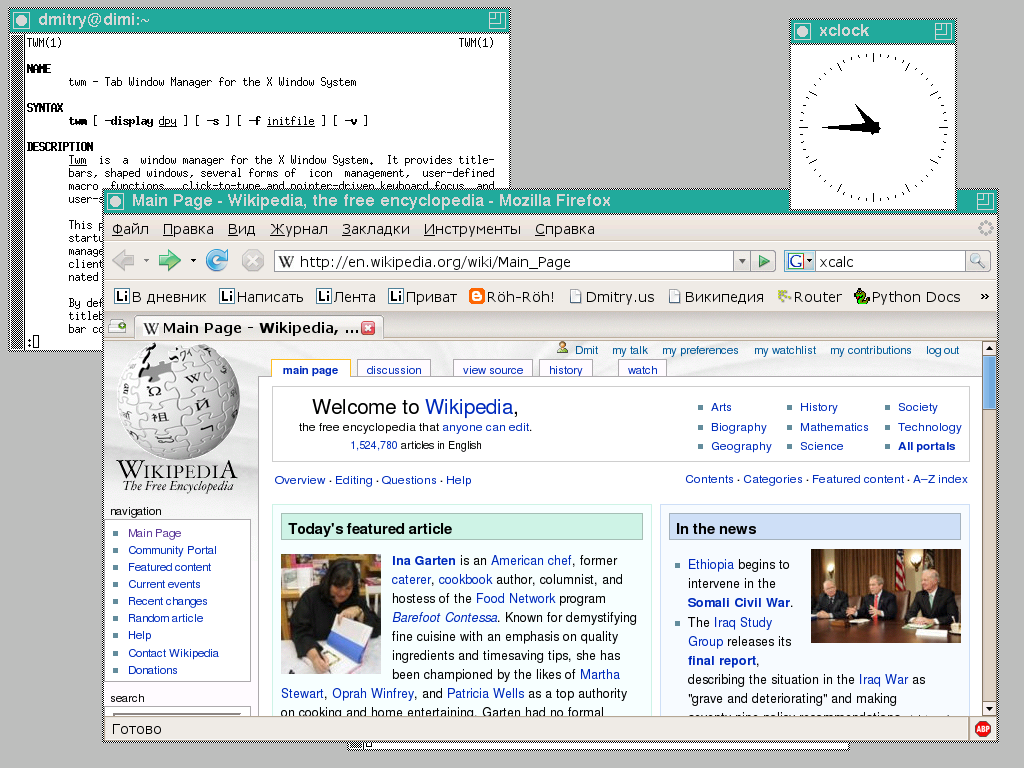
\includegraphics[width=.5\linewidth]{figures/Twm.png}
    \caption[xarch]{Twm, un window manager per X Window System \footnotemark}
\end{figure}
\footnotetext{Di Dmitry Makarov - Opera propria, CC BY-SA 4.0 \url{https://commons.wikimedia.org/w/index.php?curid=1445865}}

\paragraph{Architettura e Desktop Remoto}
% fonte: https://www.maketecheasier.com/the-x-window-system/ e wikipedia

X è una collezione di software che si posizionano tra il kernel e altri software di più alto livello detti X-clients.
X si basa su una architettura client-server dove il server è in esecuzione sulla macchina che ospita l'interfaccia grafica e il client è l'applicazione che richiede servizi grafici \cite{Scheifler1986}.
%
Questa terminologia può sembrare controintuitiva in quanto chi non ha familiarità con il sistema X potrebbe pensare che sia invertita.
In realtà il tutto deve essere visto dal punto di vista delle applicazioni: queste richiedono servizi grafici e I/O al server X.
I client possono essere locali o remoti. Ogni server X può connettersi a molteplici client.
% immagine architettura X Window System
\begin{figure}
    \centering
    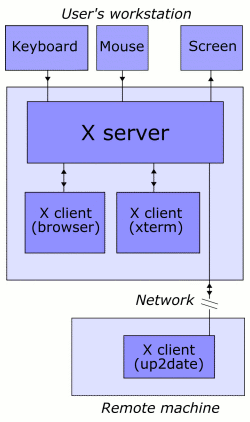
\includegraphics[width=.3\linewidth]{figures/X_client_server_example.png}
    \caption[xarch]{Esempio di architettura client-server di X Window System \footnotemark}
\end{figure}
\footnotetext{Di David Gerard, recreated by Efitu - Wikimedia Commons, CC BY-SA 3.0 \url{https://commons.wikimedia.org/w/index.php?curid=1391232}}

La comunicazione tra server e client avviene in modalità full-duplex,
ovvero entrambi possono inviare e ricevere dati contemporaneamente.
%
Lo scambio di messaggi avviene tramite il protocollo TCP/IP,
ma spesso vengono utilizzati altri canali comunicativi come Unix domain sockets o memoria condivisa \footnote{\emph{The X New Developer’s Guide: Communication Between Client and Server}: \url{https://www.x.org/wiki/guide/communication/}}.
%
Indipendentemente dal canale utilizzato, è necessario che questo sia affidabile e che garantisca l'integrità e l'ordine dei messaggi,
in quanto il protocollo X non implementa nativamente meccanismi di ritrasmissione o di ordinamento dei pacchetti.
%
Quando un client si connette a un server X, avviene una fase di handshake che stabilisce la connessione e verifica l'autenticazione del client. Successivamente, il client può inviare richieste al server, come la creazione di finestre, il disegno di elementi grafici, o la gestione dell'input. Le richieste vengono accumulate in un buffer e inviate in modo asincrono per migliorare l'efficienza della comunicazione. Il server gestisce le richieste di più client contemporaneamente, garantendo l'isolamento tra loro, ma non fornisce alcuna garanzia di ordinamento tra client differenti, a meno che non venga esplicitamente richiesto.

A differenza di altri protocolli progettati specificamente per il desktop remoto,
X è stato sviluppato principalmente per l'esecuzione remota di singole applicazioni grafiche,
piuttosto che per la gestione completa di un ambiente desktop (Desktop Environment, DE).
%
Per eseguire un intero DE in remoto, sarebbe necessario ricorrere a software aggiuntivi come X2Go.

Un'altra limitazione del protocollo X è l'assenza di meccanismi di compressione dei dati.
Questo significa che i dati grafici vengono trasmessi senza ottimizzazione,
il che può causare un utilizzo eccessivo della larghezza di banda e peggiorare le prestazioni su connessioni lente o instabili.
%
Inoltre, tutta la parte di rendering grafico è demandata alla macchina locale su richiesta del client.

\paragraph{Esempio di utilizzo di X Window System per l'esecuzione remota di applicazioni}

Per comprendere meglio il funzionamento del X Window System in un contesto di desktop remoto, consideriamo un esempio concreto:
l'esecuzione dell'applicazione di editing testuale \texttt{gedit} su un server remoto e la sua visualizzazione su un computer locale.
Questo può essere realizzato attraverso il X forwarding con ssh, utilizzando il seguente comando:

\begin{lstlisting}[caption={Connessione remota con X forwarding}, label={lst:ssh-x}, language=bash]
ssh -X user@remote_server
\end{lstlisting}

Dopo aver inserito le credenziali e stabilito la connessione, possiamo avviare l'applicazione da linea di comando come avremmo fatto localmente:

\begin{lstlisting}[caption={Esecuzione di gedit su server remoto}, label={lst:gedit}, language=bash]
gedit &
\end{lstlisting}

\paragraph{Funzionamento del protocollo}

Quando viene eseguito il codice di \Cref{lst:ssh-x},
il client e il server X avviano una procedura di handshake per stabilire il canale di comunicazione sicuro.
%
Il server X verifica che il client abbia i permessi necessari per connettersi al display locale e,
se tutto è corretto,
il client e il server negoziano parametri di comunicazione come il byte-ordering,
che permette di gestire correttamente i dati tra macchine con architetture diverse.

Dopo che l'handshake e la negoziazione dei parametri sono stati conclusi,
il client remoto \texttt{gedit} invia richieste al server X locale per creare finestre, disegnare interfacce grafiche e gestire l'input dell'utente.
%
Queste richieste vengono trasmesse attraverso il tunnel \texttt{ssh}.
%
Il client chiede inoltre al server X di intercettare gli eventi di input, come la pressione di un tasto o il movimento del mouse, e di inoltrarli al client remoto.
%
Quindi, quando l'utente interagisce con \texttt{gedit} (ad esempio digitando del testo o muovendo il mouse),
il server X cattura questi eventi e li inoltra al client remoto tramite il protocollo X11.
%
Il client elabora gli eventi e, se necessario, invia aggiornamenti grafici che vengono visualizzati sul display locale.
%
Questo flusso di comunicazione è gestito in modo asincrono, permettendo al server di accumulare richieste in un buffer e processarle in modo efficiente, ottimizzando così l'uso della rete.

\subsection{Virtual Network Computing}

Il protocollo \ac{VNC} è uno dei più diffusi per l'accesso remoto al desktop.
%
Sviluppato presso il laboratorio di ricerca Olivetti \& Oracle Research Laboratory nel 1998,
\ac{VNC} è stato inizialmente progettato per consentire l'accesso alle workstation da diversi dispositivi,
sia all'interno che all'esterno del laboratorio.
Sebbene X Window System offrisse già funzionalità simili, richiedeva che il dispositivo remoto eseguisse un server X,
che risultava spesso troppo oneroso per dispositivi con capacità di elaborazione limitate. Inoltre, X Window System era strettamente legato all'ambiente Unix \cite{richardson1998vnc}.

\ac{VNC}, al contrario, è stato concepito per essere indipendente dal sistema operativo e per garantire leggerezza nell'esecuzione.
Questo rende possibile la sua implementazione su qualsiasi dispositivo e l'accesso da qualunque altro dispositivo dotato di un client \ac{VNC},
anche poco potente.
%
Una delle caratteristiche chiave di \ac{VNC} è la semplicità del client, che non mantiene stati complessi,
permettendo una facile disconnessione e riconnessione senza compromettere lo stato del server o l'ambiente desktop.

\subsubsection{Architettura e funzionamento}

Alla base del sistema \ac{VNC} si trova il protocollo Remote Framebuffer (RFB)
\footnote{\textbf{\ac{VNC}} - \emph{Wikipedia}: \url{https://w.wiki/BoHJ}},
che opera a livello di framebuffer,
rendendolo compatibile con qualsiasi sistema operativo,
sistema di finestre o applicazione.
%
Il sistema \ac{VNC} è composto principalmente da due componenti:
il server \ac{VNC} e il client \ac{VNC}.
%
Il server è responsabile delle modifiche al framebuffer e ospita il sistema di finestre e le applicazioni,
mentre il client rappresenta l'endpoint con cui l'utente interagisce attraverso il display e i dispositivi di input \cite{richardson1998vnc}.

\paragraph{Rendering grafico}

Il sistema \ac{VNC} utilizza un metodo di rendering molto semplice, basato su una singola operazione grafica:
\begin{quote}
    "Posiziona un rettangolo di dati di pixel in una determinata posizione \emph{x}, \emph{y}."
\end{quote}
Questo approccio, pur sembrando inefficiente a prima vista, offre grande flessibilità grazie all'uso di diversi schemi di codifica dei dati grafici.
%
Ad esempio il server può ottimizzare la trasmissione di dati riciclando informazioni già presenti sullo schermo del client.
%
Se una finestra viene spostata da una posizione all'altra sul desktop,
il server \ac{VNC} invierà semplicemente una richiesta per spostare il rettangolo corrispondente dalla posizione iniziale (\texttt{x1, y1}) alla nuova posizione (\texttt{x2, y2}).
%
Inoltre, \ac{VNC} utilizza tecniche di compressione dei dati per ridurre significativamente la quantità di informazioni da trasmettere.

Un insieme di rettangoli di pixel modificati viene definito "framebuffer update".
Ogni rettangolo può essere codificato in modo diverso,
consentendo al server di scegliere il metodo di codifica più efficiente in base alla situazione.
%
A differenza di un frame video completo,
un aggiornamento del framebuffer riguarda solo la porzione di schermo modificata.
%
Gli aggiornamenti vengono inviati in modo asincrono: il server invia nuovi aggiornamenti solo quando è necessario;
questo consente di adattare la frequenza degli aggiornamenti in base agli eventi sullo schermo, alla velocità della rete e alle capacità del client \cite{richardson1998vnc}.
%
Ad esempio, se l'utente trascina una finestra su una connessione veloce con un client potente,
gli aggiornamenti saranno continui e fluidi. In caso di connessione lenta o client con risorse limitate,
il server ridurrà la frequenza degli aggiornamenti, causando un movimento meno fluido.

\paragraph{Input}

\ac{VNC} supporta un modello standard di input che include una tastiera e un dispositivo di puntamento multi-pulsante.
Il client invia eventi di input ogni volta che un tasto viene premuto o il mouse viene mosso, permettendo al server di elaborare questi eventi e aggiornare l'interfaccia di conseguenza. \cite{richardson1998vnc}.

\paragraph{Connessione e autenticazione}

Quando un client richiede la connessione a un server \ac{VNC},
il server risponde con una richiesta di autenticazione,
generalmente basata su un meccanismo di password \textit{challenge-response}.
%
Una volta autenticato, client e server negoziano parametri come la risoluzione dello schermo,
il formato dei pixel, i metodi di codifica supportati e altre impostazioni.
%
Dopo la negoziazione, la sessione viene avviata e il client richiede il primo aggiornamento del framebuffer \cite{richardson1998vnc}.

\subsection{Remote Desktop Protocol}
\label{sec:rdp}
\ac{RDP} è un protocollo proprietario sviluppato da Microsoft per l'accesso remoto a sistemi Windows.
Viene introdotto nel 1998 con Windows NT 4.0 Terminal Server Edition e successivamente integrato in tutte le versioni successive di Windows (ad eccezione delle versioni Home).

\subsubsection{Il Protocollo}
Al suo interno lo stack \ac{RDP} è composto da diversi protocolli, ognuno con un compito specifico.
\begin{itemize}
    \item \textbf{TPKT}: Anche conosciuto come \emph{ISO Transport Service on top of the TCP (RFC 1006)}, è un protocollo di trasporto che fornisce un servizio di trasporto orientato alla connessione
     Permette lo scambio di unità di dati \ac{TPDU} tra due host.
    \item \textbf{X.224}: Protocollo di livello di trasporto che fornisce servizi di sessione e di connessione. Gestisce le richieste e risposte di connessione.
    \item \textbf{T.125 MCS}: Protocollo che permette ad \ac{RDP} di gestire e comunicare attraverso più canali di comunicazione.
\end{itemize}

\begin{figure}
    \centering
    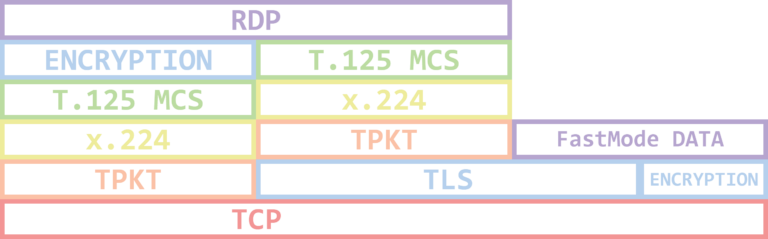
\includegraphics[width=.5\linewidth]{figures/3-protocol_stack-768x239.png}
    \caption[xarch]{Stack di protocolli \ac{RDP} \footnotemark}
\end{figure}
\footnotetext{Fonte: \url{https://www.anyviewer.com/how-to/what-is-rdp-2578.html}}

L'attività di invio e ricezione dei dati tramite lo stack \ac{RDP} segue essenzialmente lo stesso schema del modello OSI a sette livelli,
comune nelle reti \ac{LAN}.
%
I dati di un'applicazione o servizio vengono segmentati,
indirizzati a un canale, crittografati,
incapsulati e impacchettati nel protocollo di rete, per poi essere inviati al client.
%
I dati ricevuti subiscono il processo inverso: vengono decapsulati, decrittografati e, infine, resi disponibili all'applicazione.

\subsubsection{Connessione}

La fase di connessione può essere suddivisa nelle seguenti fasi:
\begin{enumerate}
    \item \textbf{Inizializazione della connessione}: Il client invia un \ac{PDU} di richiesta di connessione utilizzando il protocollo X.224. Il server risponde con un \ac{PDU} di conferm di connessione.
    In questa fase viene stabilito il protocollo di sicurezza da utilizzare.
    \item \textbf{Scambio delle Impostazioni di Base}: Tramite MCS Connect Initial \ac{PDU} e MCS Connect Response \ac{PDU},
    client e server scambiano informazioni di base come la versione del protocollo, la dimesione del desktop,
    dati riguardanti la sicurezza come il server random e il certificato e informazioni di rete come il numero di canali supportati.
    \item \textbf{Connessione dei Canali}: Il client e il server stabiliscono le connessioni individuali per ogni canale virtuale previsto nella sessione,
    tramite una serie di richieste e conferme.
    \item \textbf{Avvio della Sicurezza}: Il client invia un \ac{PDU} di scambio di sicurezza contenente un numero casuale cifrato, utile per generare le chiavi di sessione.
    Da questo punto, il traffico \ac{RDP} può essere cifrato.
    \item \textbf{Scambio delle Impostazioni di Sicurezza}: Il client invia un \ac{PDU} criptato contenente informazioni di configurazione come username,
    dominio e opzioni di compressione supportate.
    \item \textbf{Verifica della Licenza}: Questa fase verifica se il client è autorizzato a connettersi a un terminal server con un numero maggiore di connessioni simultanee.
    Se il server non ha una licenza configurata, consente fino a due connessioni.
    \item \textbf{Scambio delle Funzionalità supportate}: Il server e il client scambiano informazioni sui rispettivi tipi di capacità supportati, come codec per bitmap,
    supporto per tastiera e mouse, e configurazioni generali.
    \item \textbf{Finalizzazione della Connessione}: Il client e il server completano la connessione attraverso una serie di \ac{PDU}s per sincronizzare i rispettivi identificatori utente e definire il controllo condiviso della sessione.
    \item \textbf{Scambio dei Dati}: Una volta stabilita la connessione, il client invia dati di input (come tastiera e mouse) e riceve output grafico dal server,
    con l’opzione di utilizzare la compressione per ridurre il traffico dati.
\end{enumerate}

\subsubsection{Input e Output}
Durante una sessione \ac{RDP}, il client invia dati di input (come ad esempio mouse e tastiera) al server, mentre quest'ultimo invia al client dati di output, principalmente grafici.
Questo scambio di dati avviene attraverso due modalità: \textit{slow-path} e \textit{fast-path}:
\begin{itemize}
    \item \textbf{Slow-Path}: Questa modalità è la più completa, in cui ogni pacchetto di dati \ac{PDU} include l'intera serie di header del protocollo \ac{RDP}.
    Questo lo rende adatto per inviare dati critici che richiedono la piena gestione dei metadati, anche se aumenta la dimensione dei pacchetti trasmessi e il consumo di banda.
    \item \textbf{Fast-Path}: Riducendo o rimuovendo alcuni degli header da alcuni \ac{PDU},
    questa modalità permette di ridurre la quantità di dati trasmessi e la latenza di trasmissione.
    Inoltre così facendo riduce anche il carico di lavoro per processare i pacchetti.
    Fast-Path è comunemente usato per input a bassa priorità, come movimenti del mouse e sequenze di tasti, dove è importante minimizzare il ritardo.
\end{itemize}

\subsubsection{Canali in RDP}
\ac{RDP} si avvale di diversi canali per la trasmissione di dati. Esistono due tipi principali di canali:
\begin{itemize}
    \item \textbf{\ac{SVC}}: Limitati a 31 per connessione,
    questi canali trasportano comunicazioni essenziali tra client e server, come il canale I/O o il canale utente. Vengono instaurati durante lo "Scambio delle Impostazioni di Base" e rimangono attivi per tutta la durata della sessione.
    \item \textbf{\ac{DCV}}: Trasportati su uno specifico \ac{SVC} (chiamato \emph{DRDYNVC}),
    i \ac{DCV}, a differenza degli \ac{SVC},
    possono essere creati e distrutti liberamente durante la sessione.
    Questi canali possono essere liberamente utilizzate da sviluppatori per estendere le funzionalità di \ac{RDP}.
    Utilizzi comuni sono l'input audio (da client a server), rendering grafico e PnP.
\end{itemize}

\subsection{Parsec}
\label{sec:parsec}
Parsec è un software di desktop remoto focalizzato principalmente sul gaming. Rispetto alle tecnologie precedenti è ideato per ridurre al minimo la latenza tra il client e il server.
La capacità di offrire streaming video a bassa latenza, alta risoluzione e alto frame rate lo rende adatto non solo per il gaming ma anche per applicazioni professionali come l'editing video o la progettazione grafica.
Nasce dall'idea di utilizzare istanze GPU di Amazon Web Services per lo streaming di giochi a bassa latenza su dispositivi meno potenti e successivamente si evolve in un servizio di desktop remoto completo.
%
A differenza di alcune tecnologie sopra citate,
Parsec trasmette come flusso video un "mirror" del desktop dove è presente il server,
permettendo di visualizzare l'intero ambiente desktop e non solo singole applicazioni. Quindi parsec si comporta come se dovesse trasmettere un video.
Aggiungendo la possibilità di trasmettere input da tastiera e mouse, il client può interagire con il server come se si trovasse fisicamente davanti ad esso.

Il client Parsec è disponibile per Windows, macOS, Linux, Android, Raspberry Pi e web browser. Il server Parsec è disponibile per Windows e macOS. 

\subsubsection{Procedura di Trasmissione e Visualizzazione}

Il flusso di lavoro di Parsec per la trasmissione video si compone delle seguenti fasi:
\begin{enumerate}
    \item Cattura del frame
    \item Compressione
    \item Trasmissione
    \item Decodifica
    \item Rendering
\end{enumerate}

\paragraph{Cattura del frame}
Per la cattura del frame su Windows, Parsec utilizza la Desktop Duplication API (disponibile a partire da Windows 8.1),
che consente diretto accesso al framebuffer e permette di trasferire il frame nella memoria video della GPU.

\paragraph{Compressione}
\label{sec:compressione}
Per poter trasmettere questo flusso video ad alta risoluzione e frame rate su una rete, è necessario comprimerlo.
La compressione di un video può essere eseguita in due modi: software e hardware.
%
La compressione software è eseguita dalla CPU, mentre la compressione hardware è eseguita da un chip dedicato, come una GPU (integrata o dedicata).
%
Il vantaggio della compressione software è la compatibilità in quanto può essere eseguita su qualsiasi dispositivo, ma il suo svantaggio è il tempo impiegato per la compressione.
La compressione hardware, al contrario, è molto più veloce ma richiede un chip dedicato, che non è sempre presente su tutti i dispositivi.
%
Parsec utilizza i codec H.264 e H.265, scelti per la loro ampia compatibilità hardware così da permettere compressione hardware per qualsiasi dispositivo relativamente recente.

Per ridurre al minimo le latenza, Parsec è progettato per far si che il framebuffer,
una volta catturato, venga direttamente inviato alla GPU per essere codificato senza passare per la memoria di sistema, evitando operazioni CPU intermedie.

\paragraph{Trasmissione}
Per garantire una connessione a bassa latenza, Parsec utilizza due connessione Peer-To-Peer UDP sia per client che per host.

\paragraph{Decodifica}
Una volta ricevuto dal client, il frame compresso viene decodificato. Anche in questo caso Parsec predilige la decodifica hardware, sfruttando ASIC o GPU per ridurre al minimo la latenza.

\paragraph{Rendering}
L'ultimo passaggio della procedura è il rendering, che consiste nel visualizzare il frame decodificato sullo schermo del client. Parsec, per minimizzare i ritardi e garantire una visione fluida, utilizza la sincronizzazione verticale (V-sync) per allineare la visualizzazione del frame con il refresh rate del monitor, evitando problemi di tearing. Questo implica una sincronizzazione accurata tra i frame inviati dal server e il display del client.

\subsubsection{Latenza}
\label{sec:latenza-parsec}

Come abbiamo detto, la sfida principale di Parsec è ridurre al minimo la latenza tra il client e il server. Eseguendo tutte le operazioni sulla GPU, evitando che la CPU sia coinvolta nella compressione e decompressione dei frame, Parsec riesce a ridurre la latenza a pochi millisecondi. Inoltre, utilizzando connessioni Peer-To-Peer UDP, Parsec evita i ritardi dovuti ai server intermedi, garantendo una connessione diretta tra client e host. Una limitazione che Parsec non può superare è la latenza intrinseca della rete, che può variare in base alla qualità della connessione e alla distanza geografica tra client e server. Fortunatamente negli ultimi anni la diffusione di connessioni ad alta velocità e a bassa latenza è aumentata notevolmente, sopratutto con l'aumento di connessioni Fiber To The Home (FTTH).

\subsubsection{Altri Utilizzi}
Grazie alla sua capacità di trasmettere video ad alta risoluzione e frame rate, Parsec è spesso utilizzato non solo per cloud gaming o desktop remoto Over The Internet, ma anche per Local Game Streaming. Questo consiste nell'avere una macchina potente da cui potersi collegare da altri dispositivi meno potenti, come una smart TV, così da poter avere un'esperienza di gioco di alta qualità su un dispositivo che altrimenti non sarebbe in grado di supportare i giochi più recenti.

\subsection{Altre Tecnologie Rilevanti}
Ci sono altri protocolli proprietari che meritano una menzione, come lo storico Team-Viewer o AnyDesk, che offrono funzionalità di desktop remoto per utenti meno esperti grazie ad un setup minimo evitando l'apertura di porte. Purtroppo le informazioni sul funzionamento di questi sono molto limitate e non è possibile approfondire ulteriormente.

Con la diffusione del local game streaming, sono nate altre tecnologie simili a Parsec, che offrono funzionalità simili ma con alcune differenze. Tra queste troviamo Steam Link (sviluppato da Valve), Rainway e Moonlight.

NVIDIA, con la tecnologia Gamestream, permetteva di trasmettere il flusso video di un gioco da un computer con una GPU NVIDIA ad un dispositivo NVIDIA Shield. Per poter utilizzare questa funzione, e il server messo a disposizione dai driver NVIDIA, e ricevere questo flusso su ogni dispositivo, la community open-source ha sviluppato Moonlight, un client compatibile con qualsiasi dispositivo Android, iOS, Windows, macOS e Linux, in grado di ricevere il flusso video da un server NVIDIA Gamestream.

Quando nel 2022 NVIDIA ha deciso di rimuovere il supporto per i server Gamestream, la community ha sviluppato Sunshine, un server open-source in grado di trasmettere il flusso video di un gioco da un computer con una qualsiasi GPU (Gamestream era limitato a NVIDIA) ad un client Moonlight.
Con il passare del tempo Sunshine è migliorato notevolmente, ed utilizzando un concetto molto simile a quello di Parsec, è in grado di ottenere latenze molto basse, rendendolo adatto non solo per il gaming, ma anche per applicazioni professionali. Inoltre la sua natura open-source e i continui impegni della community a migliorarlo, lo rendono migliore di molte soluzioni proprietarie. Sunshine infatti, rispetto a Parsec, è disponibile anche su Linux, oltre che su Windows e macOS. Supporta inoltre numerosi metodi di cattura e permette all'utente di modificare parametri come la qualità del video, la risoluzione e il frame rate, in base alle necessità e alla potenza del computer.

\chapter{Sviluppi e Applicazioni Attuali delle Tecnologie di Desktop Remoto}
\label{chap:current-applications}
% -- VDI, Cloud Gaming, Smart working, Assistenza Remota, DaaS, Applicazioni virtualizzate

Negli ultimi anni, le tecnologie di desktop remoto si sono evolute da semplici strumenti per l’accesso remoto a sistemi aziendali fino a diventare soluzioni fondamentali in numerosi ambiti. Le applicazioni attuali delle tecnologie di desktop remoto non solo supportano i lavoratori e le aziende nella gestione delle loro operazioni quotidiane, ma sono diventate fondamentali anche per l’intrattenimento, soprattutto in ambito videoludico.

Questo capitolo esplora le principali applicazioni delle tecnologie di desktop remoto di cui si è parlato nel capitolo precedente, analizzando come queste tecnologie vengono utilizzate in diversi scenari e settori.

\section{Assistenza Remota}
\label{sec:remote-assistance}

L'assistenza remota rappresenta una delle applicazioni più diffuse delle tecnologie di desktop remoto, consentendo a un operatore tecnico di visualizzare e, all'occorrenza, controllare il desktop di un utente remoto. Questo approccio trova applicazione in diversi ambiti, sia professionali che personali, grazie alla possibilità di intervenire su una postazione senza la necessità di spostamenti fisici, riducendo così tempi e costi operativi in modo significativo.

Nel contesto aziendale, l'assistenza remota permette al personale tecnico di fornire supporto ai dipendenti senza doversi spostare fisicamente tra gli uffici o recarsi presso le sedi dei clienti. Tale supporto risulta particolarmente utile per le aziende che vendono software, poiché i tecnici possono utilizzare strumenti di desktop remoto per mostrare ai clienti l'uso corretto di un'applicazione o per risolvere eventuali problemi in tempo reale. 

Anche in ambito domestico, l'assistenza remota è ampiamente utilizzata per risolvere problematiche informatiche a distanza. Un tecnico autorizzato, o anche un conoscente, può accedere al dispositivo dell’utente per fornire supporto tramite software specifici come \textit{Quick Assist} (che utilizza RDP, vedi \ref{sec:rdp}), preinstallato sui sistemi Windows 10 e 11.



\section{Infrastructure as a Service}
\label{sec:iaas}
Un possibile e diffuso utilizzo delle tecnologie di desktop remoto è il suo impiego all'interno di servizi di cloud computing, in particolare nell'ambito dell'\ac{IaaS}.
Infrastructure as a Service è un termine che indica un modello di servizio dove un fornitore di servizi cloud mette a disposizione degli utenti risorse hardware virtualizzate, come server, reti, spazio di archiviazione e sistemi operativi, su richiesta. In poche parole permette all'utente di noleggiare un'infrastruttura IT completa, senza dover acquistare o gestire fisicamente hardware e strutture di rete.

\subsection{Principali Caratteristiche di Infrastructure as a Service}
Un provider di servizi \ac{IaaS} mette a disposizione dell'utente l'hardware (tipicamente virtualizzato), i servizi amministrativi per la gestione delle risorse e una piattaforma per poter eseguire applicativi (come sistemi operativi).
Come ogni servizio di cloud computing, \ac{IaaS} ricade sotto queste cinque caratteristiche fondamentali\cite{bhardwaj2010cloud}:
\begin{itemize}
    \item \textbf{Self-service on demand}: l'utente può richiedere e configurare risorse in modo autonomo, senza l'intervento del fornitore;
    \item \textbf{Ampio accesso alla rete}: le risorse sono accessibili tramite Internet o una rete privata;
    \item \textbf{Risorse condivise}: le risorse sono condivise tra più utenti, garantendo efficienza e scalabilità;
    \item \textbf{Risorse scalabili}: le risorse possono essere allocate e deallocate rapidamente in base alle esigenze;
    \item \textbf{Misurabilità del servizio}: l'uso delle risorse può essere monitorato e misurato, consentendo una gestione efficiente dei costi.
\end{itemize}
Questo porta a una serie di vantaggi per le aziende o gli utenti che ne fanno uso, tra cui\cite{bhardwaj2010cloud}:
\begin{itemize}
    \item \textbf{Costo incrementale}: l'utente paga solo per le risorse effettivamente utilizzate e per il tempo di utilizzo;
    \item \textbf{Ampio storage}: possibilità di archiviare grandi quantità di dati in modo scalabile;
    \item \textbf{Mantenimento semplificato}: il fornitore si occupa della manutenzione dell'hardware e degli aggiornamenti software (almeno quelli di base);
    \item \textbf{Accesso globale}: le risorse sono accessibili da qualsiasi luogo connesso a Internet;
    \item \textbf{Flessibilità e scalabilità}: le risorse possono essere adattate alle esigenze specifiche dell'applicazione e aumentate o ridotte rapidamente;
\end{itemize}

\subsection{Provider e Cliente}
\label{subsec:provider_cliente}
Nel modello \ac{IaaS}, gli attori principali sono il \textbf{Provider} e il \textbf{Cliente}. Il Provider è responsabile della gestione dell'infrastruttura fisica e virtuale, come server, macchine virtuali, rete e sistemi di archiviazione. Inoltre si occupa della manutenzione e degli aggiornamenti dei software e sistema operativo\cite{bhardwaj2010cloud}.
Il livello di servizio viene formalizzato in specifici \ac{SLA}, che stabiliscono standard di disponibilità e prestazioni.

Il Cliente invece si occupa della gestione delle proprie applicazioni e dati all'interno dell'infrastruttura fornita\cite{bhardwaj2010cloud}.

\subsection{Desktop as a Service}
\label{subsec:daas}
Desktop as a Service (DaaS) è un modello di cloud computing in cui un provider fornisce desktop virtuali accessibili via Internet. A differenza di \ac{IaaS}, che mette a disposizione risorse infrastrutturali di base come server e storage su cui un cliente può costruire e gestire autonomamente il proprio ambiente IT, DaaS offre un ambiente desktop pronto all'uso, ideale per utenti finali che necessitano di un accesso immediato a un sistema completo senza doversi occupare di configurazioni hardware.

\subsubsection{Similitudini e differenze con IaaS}
Entrambi i modelli offrono scalabilità e gestione centralizzata, permettendo di pagare solo per le risorse effettivamente utilizzate. Tuttavia, mentre in \ac{IaaS} il Cliente è responsabile del sistema operativo e delle applicazioni, in DaaS il provider gestisce interamente il desktop, inclusi aggiornamenti e sicurezza. Questo rende DaaS una soluzione più semplice e immediata, particolarmente utile per scenari di lavoro remoto.

\subsubsection{Vantaggi di DaaS e Desktop Remoto}
DaaS offre accessibilità da qualsiasi dispositivo, maggiore sicurezza dei dati grazie alla gestione centralizzata, e una riduzione dei costi di manutenzione. In sintesi, \ac{IaaS} è ideale per chi necessita di infrastrutture flessibili, mentre DaaS è pensato per chi cerca un desktop virtuale pronto all'uso.

Rispetto ad una soluzione \ac{IaaS}, DaaS potrebbe essere meno flessibile per quanto riguarda la scelta del sistema operativo e applicazioni, ma guadagna in semplicità e immediatezza d'uso.
Prendiamo in esempio un 3D artist che necessita di un ambiente di lavoro con una GPU potente per eseguire rendering complessi. Con una soluzione \ac{IaaS}, l'artista potrebbe configurare un server con una GPU dedicata e installare il software necessario. Con DaaS, invece, potrebbe accedere a un desktop virtuale già configurato con le specifiche richieste, senza dover gestire l'infrastruttura sottostante.
Abbinando un sistema scalabile, immediato e on-demand come DaaS con una tecnologia di desktop remoto a bassa latenza, DaaS diventa un'alternativa competitiva rispetto all'acquisto di hardware fisico costoso e alla gestione di un'infrastruttura IT complessa.

Inoltre bisogna considerare che un utente può accedere al proprio desktop virtuale da qualsiasi dispositivo connesso a Internet.
Poter accedere da un laptop in treno, successivamente dalla workstation in ufficio e infine dal tablet a casa senza mai perdere lo stato dell'ambiente di lavoro, è un vantaggio che non può essere sottovalutato, sopratutto in un'epoca in cui il lavoro remoto è sempre più diffuso.

\section{Cloud Gaming}
\label{sec:cloud-gaming}
L'industria dei videogiochi ha visto una enorme crescita negli ultimi anni, sopratutto per quanto riguarda la potenza di calcolo richiesta per eseguire i giochi più recenti. Molti di questi, sopratutto i tripla A (termine utilizzato per indicare giochi con un budget di sviluppo molto alto), utilizzano modelli 3D complessi, texture ad alta risoluzione e tecnologie come il ray tracing, che migliorano notevolmente la qualità grafica ma richiedono una potenza di calcolo molto elevata.
Hardware in grado di supportare questi giochi può essere molto costoso, e non tutti gli utenti possono permettersi di acquistare una GPU di fascia alta o un computer con specifiche tecniche elevate.
Per questo ed altri motivi che vedremo in seguito, il cloud gaming è diventato una soluzione sempre più popolare.
Cloud Gaming, anche noto come \ac{GaaS}, è un servizio di cloud computing che permette agli utenti di giocare a videogiochi su server remoti, trasmettendo il flusso video del gioco a bassa latenza su dispositivi client di vario tipo. \cite{HARLE2023}

\subsection{Principio di Funzionamento}
\label{subsec:funzionamento}

Il funzionamento del cloud gaming si basa sull'architettura del cloud computing, che permette di eseguire i giochi in remoto su server e di trasmettere in streaming il video generato all'utente finale. Questo servizio sfrutta i modelli di servizio \ac{IaaS}, PaaS e SaaS per offrire un servizio scalabile e facile da utilizzare.

\subsubsection{Infrastructure as a Service (IaaS)}
In GaaS, i provider utilizzano \ac{IaaS} per fornire l'infrastruttura hardware necessaria. Le risorse includono server con CPU e GPU potenti in grado di eseguire i giochi più "pesanti". Grazie a IaaS, i provider possono gestire dinamicamente l'allocazione delle risorse, adattandole in tempo reale alla domanda e ottimizzando i costi. Inoltre potendo distribuire i server in data center in tutto il mondo, è possibile ridurre la latenza e distribuire il carico in modo efficiente \cite{HARLE2023}.

\subsubsection{Platform as a Service (PaaS)}
PaaS può essere utilizzato dagli sviluppatori di videogiochi per avere un ambiente stabile e scalabile su cui sviluppare e testare i giochi senza doversi preoccupare dell'hardware sottostante. I provider forniscono piattaforme con librerie, strumenti e software necessari per lo sviluppo di giochi \cite{HARLE2023}.

\subsubsection{Software as a Service (SaaS)}
Quando si parla di cloud gaming, il livello SaaS è l'ultimo passo per fornire i giochi agli utenti finali. I servizi SaaS permettono all'utente di avviare un gioco direttamente dalla piattaforma di streaming (ad esempio dal browser o da un applicativo installato sul thin-client) senza bisogno di scaricare ed installare pesanti file di gioco. È proprio qui che le tecnologie di desktop virtuale e remoto entrano in gioco, permettendo di trasmettere il flusso video del gioco dal server IaaS al dispositivo dell'utente ed inviare input da tastiera e mouse al server \cite{HARLE2023}.

\subsection{Tecnologie di streaming}
\label{subsec:streaming-tech}
Per ridurre al minimo la latenza, aumentare la qualità del video e garantire un'esperienza di gioco fluida, i provider di cloud gaming utilizzano tecnologie di streaming avanzate.
Alcune di queste tecnologie includono:

\paragraph{Streaming a Bitrate Adattivo} Questa tecnologia permette di adattare la qualità del video in base allo scenario presente e alla larghezza di banda disponibile. È molto utile in situazioni in cui la connessione Internet è instabile, permettendo di mantenere un'esperienza di gioco fluida anche in presenza di fluttuazioni della larghezza di banda.

\paragraph{H.264 e H.265} Questi codec sono utilizzati per comprimere il flusso video in modo efficiente, riducendo la quantità di dati trasmessi e garantendo una qualità video elevata. Vedi \ref{sec:compressione}.

\paragraph{QUIC} Quick UDP Internet Connections (QUIC) è un protocollo di trasporto sviluppato da Google che permette di ridurre la latenza e migliorare la sicurezza delle connessioni Internet. Queste caratteristiche lo rendono particolarmente adatto per il cloud gaming.

\subsection{Vantaggi e Svantaggi}
Il Cloud Gaming condivide molti degli stessi vantaggi e svantaggi dei servizi IaaS e DaaS, con alcune caratteristiche specifiche. Vediamo insieme i principali vantaggi e svantaggi del cloud gaming.

\subsubsection{Vantaggi}
\paragraph{Facilità d'uso} Uno degli aspetti più apprezzati del cloud gaming è la facilità d'uso. Gli utenti devono semplicemente scaricare un applicativo o accedere ad una pagina Web da un qualsiasi dispositivo connesso a Internet e possono iniziare a giocare immediatamente, senza dover installare o configurare software aggiuntivo.
\paragraph{Comptaibilità multipiattaforma} Una grande limitazione nell'industria videoludica sta proprio nella compatibilità dei giochi con i vari sistemi operativi. Windows è il leader indiscusso per quanto riguarda il gaming e questo limita molto la quantità di dispositivi su cui è possibile giocare. Il cloud gaming d'altro canto permette di giocare ad un qualsiasi gioco presente sulla piattaforma di streaming, su un qualsiasi dispositivo compatibile con il client di streaming (che risulta molto più semplice da sviluppare rispetto ad un gioco completo).
\paragraph{Riduzione dei costi} La possibilità di avere accesso ad hardware potente grazie ad un piano di abbonamento mensile o ad utilizzo, abbassa la barriera di ingresso per i giocatori che non possono permettersi di acquistare componenti hardware costosi.
\paragraph{Prevenzione di pirateria} Essendo i giochi eseguiti e archiviati sui server del provider, è molto più difficile, se non impossibile, per un utente eseguire una copia non autorizzata del gioco.
\paragraph{Manutenzione ed aggiornamenti} Le piattaforme di cloud gaming possono applicare aggiornamenti e patch in modo centralizzato, garantendo che tutti gli utenti abbiano sempre accesso alla versione più recente del gioco. Inoltre, la manutenzione dell'hardware è a carico del provider, riducendo i costi e i tempi di inattività per l'utente.

\subsubsection{Svantaggi}
\paragraph{Latenza} Per quanto fino ad ora abbiamo parlato di come tecnologie recenti abbiamo portato la latenza a livelli impensabili fino a qualche anno fa, questa rimane comunque un problema per il cloud gaming. Anche se molto bassa, quando si parla di gaming, anche pochi millisecondi possono fare la differenza. In giochi \ac{FPS}, la reattività è fondamentale, sopratutto in multiplayer, dove pochi millisecondi di latenza in meno danno un vantaggio competitivo considerevole. Purtroppo la latenza è un problema intrinseco del cloud gaming, e nonostante i continui miglioramenti, non può essere completamente eliminata. Sia chiaro però che i giochi \ac{FPS} sono un caso limite; per la maggior parte dei giochi, la latenza è più che accettabile e non influisce sull'esperienza di gioco, anche se queste sono valutazioni molto soggettive.
\paragraph{Larghezza di banda e Requisiti di connessione} Il cloud gaming richiede una connessione relativamente veloce e stabile per garantire un'esperienza di gioco fluida. Lo scenario ideale sarebbe una connessione cablata e un contratto FTTH in quanto in questo modo la banda è garantita e la latenza è molto bassa. A partire dal 2020, secondo Steam Hardware Survey\footnote{Steam Hardware Survey: \url{https://store.steampowered.com/hwsurvey/}}, la percentuale di utenti che utilizzano un monitor con risoluzione 1080p è scesa dal 64.58\% al 57.32\% mentre la percentuale di utenti con monitor 1440p è salita dal 4.92\% al 19.71\% (dati di ottobre 2019 e ottobre 2024). Questo significa che sempre più utenti stanno adottando monitor con risoluzioni più alte, che richiedono un bitrate maggiore per garantire la stessa qualità video.

\subsection{Principali Servizi di Cloud Gaming}
In una industria redditizia come quella dei videogiochi, in cui il valore del mercato globale è stimato a circa 184 miliardi di dollari nel 2023 secondo \href{https://www.gamesindustry.biz/gamesindustrybiz-presents-the-year-in-number-2023}{GameIndustry.biz}, non sorprende che molte aziende tech abbiano investito nel cloud gaming. Di seguito sono elencati alcuni dei principali servizi di cloud gaming attualmente disponibili sul mercato.

\subsubsection{NVIDIA GeForce Now}
GeForce Now è probabilmente il leader del mercato del cloud gaming. NVIDIA, nota azienda produttrice di GPU, lancia NVIDIA GeForce Now (precedentemente chiamato NVIDIA Grid) nel 2013, come software beta per i dispositivi Shield. Viene poi rilasciato ufficialmente nel 2015. Questo servizio permetteva agli utenti abbonati di avere accesso illimitato ad una libreria limitata di giochi disponibile nei server NVIDIA.
Nel 2017, NVIDIA lancia GeForce Now per Windows e Mac, e successivamente, nel 2019, per Android. Nel 2019 viene cambiato il modello di business; ora l'utente non pagava più un abbonamento mensile per avere accesso ad una libreria di giochi, ma poteva giocare ai propri giochi acquistati su Steam, Epic Games Store, Uplay e altri store, su server NVIDIA. I piani di abbonamento differiscono per il tempo di gioco massimo continuativo e per la potenza della GPU a disposizione.
Il servizio esce completamente dalla fase beta nel 2020.
GeForce Now è rinomato per la sua bassa latenza e possibilità di trasmettere video ad alte risoluzioni (fino a 4K) e frame rate rispetto ad altri servizi di cloud gaming.

\subsubsection{Xbox Cloud Gaming}
Xbox Cloud Gaming, precedentemente noto come Project xCloud, è un servizio di cloud gaming sviluppato da Microsoft e incluso nel servizio Xbox Game Pass Ultimate. Viene rilasciato in beta nel 2019 e ufficialmente nel 2020. Il modello di business consiste nel pagare un abbonamento mensile per avere accesso ad una libreria di giochi disponibili su Xbox Game Pass, che include alcuni titoli di Xbox e PC. Il servizio è disponibile su dispositivi Android, iOS, Windows, Mac, browser e molti altri dispositivi.

\subsubsection{Playstation Now}
Playstation Now è il servizio di cloud gaming di Sony, disponibile per PlayStation 4, PlayStation 5, PC e dispositivi Android. Il servizio permette di giocare a una vasta libreria di giochi PlayStation 2, 3 e 4 in streaming, senza la necessità di scaricare i giochi. Il servizio è stato ora unito a PlayStation Plus, il servizio di abbonamento di Sony.

\subsubsection{Amazon Luna}
Amazon Luna è il servizio di cloud gaming di Amazon, lanciato nel 2020. L'abbonamento è simile a quello di Xbox Cloud Gaming o PlayStation Now, con una libreria di giochi disponibili per gli abbonati. Il servizio è disponibile su dispositivi Fire TV, PC, Mac, iOS e Android.

\subsubsection{Google Stadia}
Google Stadia è stato un servizio di cloud gaming sviluppato e gestito da Google, lanciato nel novembre 2019 e chiuso nel gennaio 2023. L'abbonamento mensile offriva una selezione di giochi gratuiti e sconti esclusivi. Gli utenti della versione gratuita, invece, potevano giocare fino a 1080p senza costi aggiuntivi, limitandosi a comprare i giochi singolarmente.
A differenza di altri servizi, Google aveva progettato un controller Stadia specifico, che si connetteva direttamente ai server tramite Wi-Fi per ridurre la latenza di input.

Nonostante l'innovatività delle sue funzioni, Stadia ha incontrato critiche per la limitata disponibilità di giochi e la mancanza di titoli esclusivi. Di conseguenza, Google ha annunciato la chiusura della piattaforma a gennaio 2023, offrendo rimborsi per gli acquisti di hardware e software effettuati tramite il proprio store.


%----------------------------------------------


\chapter{Prospettive e Sviluppi futuri del Desktop Remoto}
% -- VR/AR, 5G,

% -- IA upscaling per ridurre latenza, Edge Computing, Fog Computing, AR VR, Blockchain?

\section{5G nelle applicazioni di Desktop Remoto}
\label{sec:5g}

Il 5G è la quinta generazione di tecnologia per le reti cellulari che promette di rivoluzionare le comunicazioni grazie a velocità di trasmissione elevate, latenza minima e capacità di connettere simultaneamente un numero elevato di dispositivi. Queste caratteristiche lo rendono particolarmente adatto per le applicazioni di desktop remoto, dove la reattività e l'affidabilità, come abbiamo visto fino ad ora, sono cruciali per l'esperienza dell'utente finale.

\subsection{Miglioramenti nelle Prestazioni del Desktop Remoto}

Le reti 5G offrono una serie di vantaggi rispetto alle tecnologie precedenti, come il 4G. Promettono latenze più basse rispetto alle reti 4G, fino a 1 ms, e velocità di trasmissione fino a 10 Gbps \cite{Dangi2021}. 

Le reti 5G, con la loro capacità di fornire latenze estremamente ridotte e velocità di trasmissione fino a 20 Gbps, possono migliorare notevolmente le applicazioni di desktop remoto in ambiti professionali, educativi e di intrattenimento. In particolare, il supporto alle comunicazioni ultra-affidabili e a bassa latenza (URLLC) permette di ottenere una maggiore fluidità nell’interazione, rendendo l’esperienza di utilizzo simile a quella offerta da una connessione locale \cite{Dangi2021, Sahu2024}. Questo potrebbe risolvere o ridurre significativamente i problemi di cui parlavamo in \ref{sec:latenza-parsec}.

Il 5G introduce inoltre un'architettura basata su tecnologie come Massive MIMO (Multiple Input Multiple Output) e il beamforming, che consentono di migliorare la copertura e la capacità della rete, riducendo l'interferenza e migliorando la qualità della connessione in ambienti densi di dispositivi \cite{Dangi2021}. Grazie a questi sviluppi, le applicazioni di desktop remoto possono beneficiare di connessioni più stabili e reattive, anche in situazioni di mobilità o in aree metropolitane densamente popolate.

Infatti attualmente l'utilizzo di desktop remoto in mobilità è limitato dalla qualità della connessione, che spesso non è in grado di garantire una latenza bassa, una velocità di trasmissione elevata e una stabilità tale da garantire un'esperienza utente soddisfacente. Il 5G grazie alle caratteristiche di cui sopra, supera queste limitazioni, estendendo le possibilità di utilizzo del desktop remoto anche in mobilità, ad esempio durante gli spostamenti o in situazioni in cui una connessione Wi-Fi non è disponibile.

\subsection{Impatto del 5G su Sicurezza e Affidabilità nel Desktop Remoto}

Oltre alle prestazioni, il 5G introduce nuove sfide e opportunità per la sicurezza delle applicazioni di desktop remoto. Le reti 5G devono affrontare rischi legati alla sicurezza, come gli attacchi informatici e la protezione della privacy, soprattutto considerando l’elevato numero di dispositivi e connessioni simultanee. Tuttavia, le funzionalità avanzate di slicing di rete offerte dal 5G permettono di creare segmenti di rete virtuali con requisiti di sicurezza specifici per le applicazioni di desktop remoto, rendendo possibile una gestione più efficace delle risorse e una maggiore protezione dei dati sensibili \cite{Dangi2021}.

La sicurezza rimane dunque un aspetto critico, poiché le applicazioni di desktop remoto richiedono un livello elevato di protezione per prevenire accessi non autorizzati e garantire l'integrità dei dati. Le reti 5G possono sfruttare tecniche avanzate come l'autenticazione basata su AI e la crittografia end-to-end per aumentare la sicurezza dei sistemi remoti \cite{Sahu2024}.

%----------------------------------------------

\section{Applicazioni del Desktop Remoto in Virtual Reality e Augmented Reality}

La virtual reality (VR) e la augmented reality (AR) sono due tecnologie innovative nell'interazione uomo-macchina. La VR permette di immergere completamente l'utente in un ambiente digitale simulato, isolando l'utente dal mondo fisico. L'AR, invece, sovrappone elementi digitali al mondo reale, aumentando, per l'appunto, la realtà, integrando informazioni digitali con l'ambiente fisico circostante. Gli \textit{Head-Worn Displays} (HWD), sono dispositivi indossabili che proiettano contenuti direttamente nel campo visivo dell'utente, costituiscono il fulcro di queste applicazioni \cite{pavanatto2021, frontiers2023}.

\subsection{Integrazione di Desktop Virtuali in Virtual Reality e Augmented Reality}

Un'applicazione promettente delle tecnologie di VR e AR è l'integrazione con i desktop virtuali e monitor virtuali. Questi ultimi sono delle superfici bidimensionali virtuali, che simulano l'aspetto e il funzionamento di un monitor fisico, ma con una flessibilità superiore\cite{pavanatto2021, frontiers2023}.
% immagine presa dal paper pavanatto2021
\begin{figure}
    \centering
    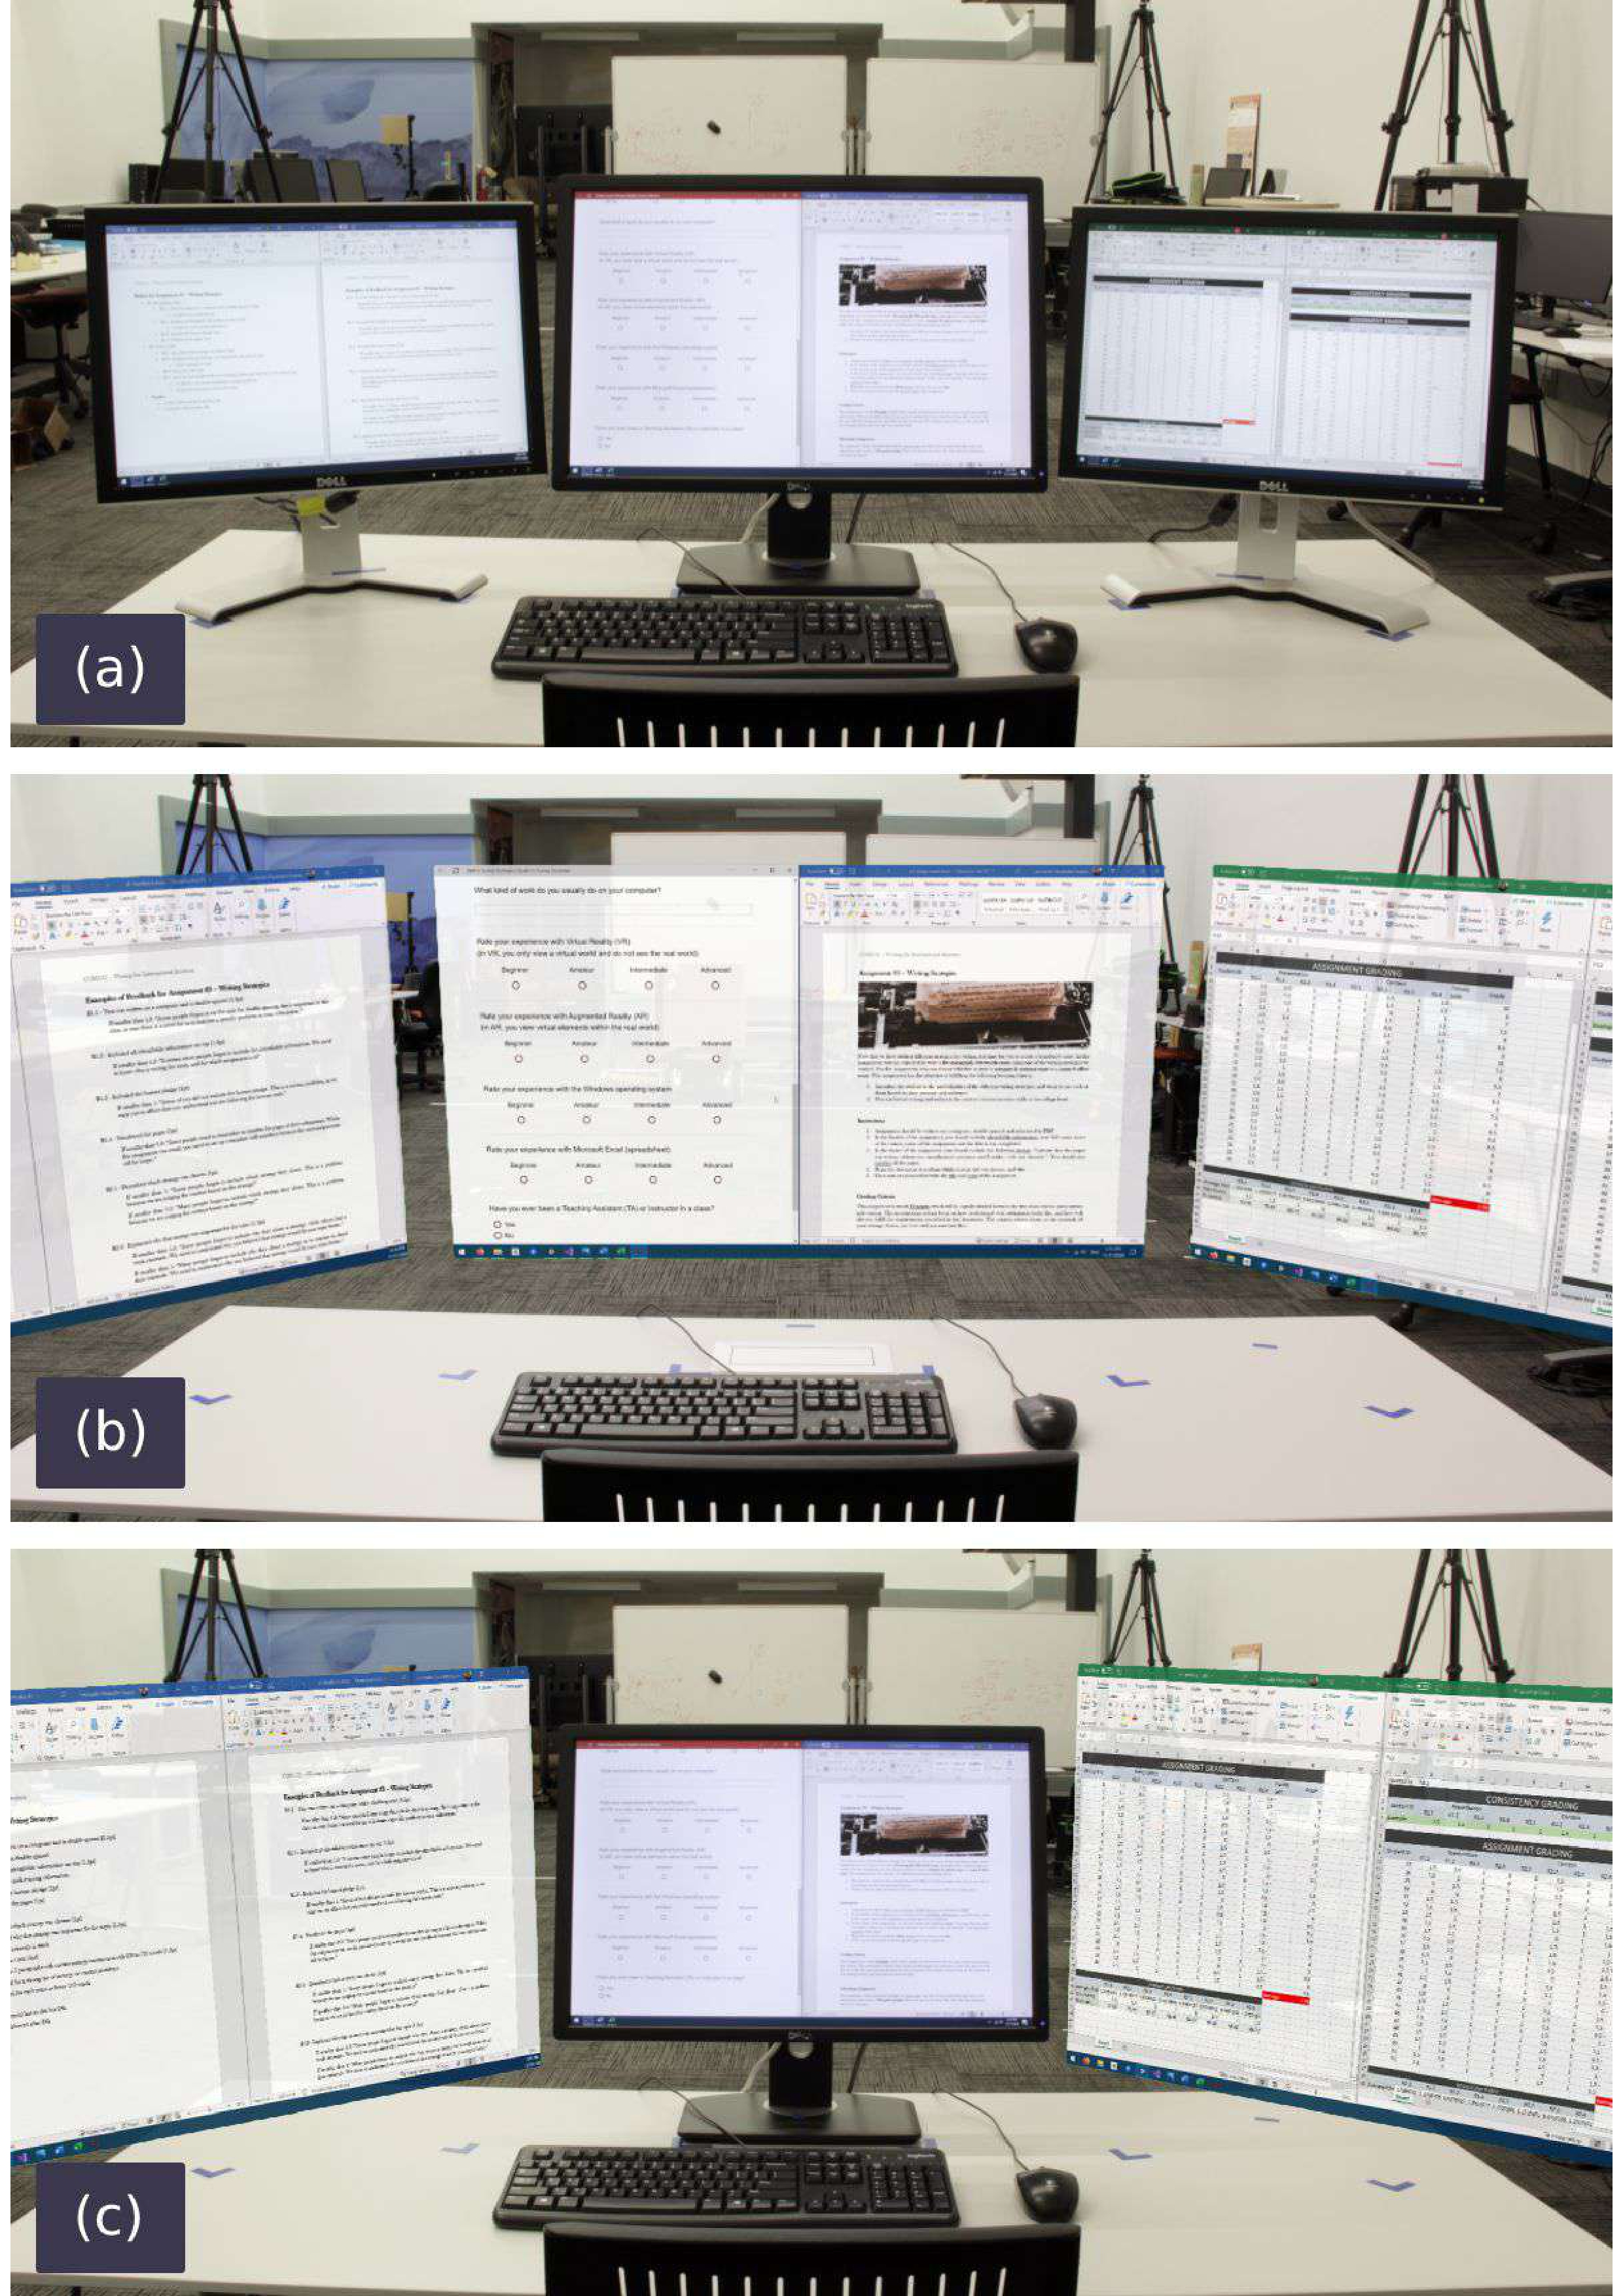
\includegraphics[width=.4\linewidth]{figures/virtual_monitors.jpg}
    \caption[xarch]{Esempio di tre modalità di visualizzazione di monitor. Dall'alto verso il basso: tre monitor fisici, tre monitor virtuali, un monitor fisico e due virtuali. Fonte \cite{pavanatto2021}}
\end{figure}

I monitor virtuali offrono diversi vantaggi teorici. In primo luogo, eliminano i vincoli fisici dei monitor tradizionali, fornendo all'utente un'area di lavoro completamente personalizzabile. Questi possono essere personalizzati a piacere, modificando grandezza, proporzione, distanza e posizione. Potenzialmente possono essere aggiunti un numero infinito di monitor, permettendo all'utente di avere un'area di lavoro molto più grande di quella fisica.
L'adozione di HWD può permettere di abbattere i costi in quanto il costo monetario non scala proporzionalmente rispetto al numero di monitor utilizzati come invece accadrebbe con l'utilizzo di monitor fisici \cite{frontiers2023}.

Inoltre, i monitor virtuali possono aumentare la privacy e la sicurezza, poiché il contenuto proiettato è visibile solo all'utente che indossa l'HWD \cite{pavanatto2021}.

Nonostante il loro potenziale, i desktop virtuali presentano ancora limitazioni significative. Gli studi condotti in \cite{pavanatto2021, frontiers2023} evidenziano come la risoluzione ridotta e il campo visivo ristretto degli attuali HWD compromettano la leggibilità e la qualità visiva rispetto ai monitor fisici. Questi problemi diventano particolarmente evidenti durante sessioni di lavoro prolungate, dove l'affaticamento visivo e il disagio fisico, dovuti al movimento frequente della testa, rappresentano ostacoli notevoli.

Inoltre, il design ergonomico degli HWD gioca un ruolo cruciale: molti dispositivi attuali risultano scomodi per un uso prolungato, richiedendo ulteriori miglioramenti nella distribuzione del peso e nell'adattamento alle caratteristiche fisiche degli utenti \cite{frontiers2023}. La difficoltà nell'integrare elementi fisici, come la tastiera, con l'ambiente virtuale rappresenta un ulteriore limite, che influisce negativamente sulla produttività.

Con l'avanzare della tecnologia, questi problemi potrebbero essere risolti, tramite l'utilizzo di headset più leggeri ed ergonomici, con l'aumento del framerate e della risoluzione. Bisogna inoltre sottolineare come l'esperienza utente sia estremamente soggettiva, e individui meno sensibili potrebbero non riscontrare questi problemi con i dispositivi attualmente disponibili.

Alla luce di quanto esposto anche in questo contesto, le tecnologie di desktop remoto possono giocare un ruolo cruciale al fine di fornire un'esperienza utente ottimale. L'utilizzo di dispositivi VR standalone come il Meta Quest 3, combinati con soluzioni di desktop remoto a bassa latenza, permetterebbe il controllo di un computer connesso da qualsiasi luogo. In combinazione ad altre tecnologie come le reti 5G \ref{sec:5g}, l'adozione di HWD potrebbe permettere agli utenti l'utilizzo di setup multi-schermo virtuale in mobilità, ad esempio durante viaggi o spostamenti.

%----------------------------------------------

\section{Smart Working: Definizione e Impatto della Pandemia di COVID-19 nel contesto Odierno}

Smart Working \footnote{\emph{Smart Working} - \emph{Treccani}: \url{https://www.treccani.it/vocabolario/smart-working_(Neologismi)/}}, noto anche come lavoro agile o lavoro da remoto, è un neologismo che indica una modalità di lavoro flessibile finalizzata ad aumentare la produttività e il benessere dei lavoratori. Questa è una modalità lavorativa che consente ai dipendenti di svolgere le proprie attività al di fuori dell’ambiente aziendale tradizionale, sfruttando tecnologie digitali e di comunicazione per connettersi con colleghi e superiori.

Anche se questa modalità era già utilizzata in precedenza, la pandemia di COVID-19 ha accelerato di molto la sua adozione. Quando le restrizioni legate alla pandemia hanno reso impossibile o poco sicuro il lavoro in ufficio, molte aziende hanno dovuto adottare il lavoro da remoto per garantire la continuità delle attività\cite{urbaniec2022}.

\paragraph{Vantaggi dello Smart Working}
Lo smart working ha permesso alle aziende di aumentare la flessibilità organizzativa, riducendo i costi di gestione degli spazi fisici e migliorando la gestione delle risorse umane. Per i dipendenti, ha significato una maggiore autonomia e un miglior bilanciamento tra vita privata e lavoro, grazie alla riduzione dei tempi di pendolarismo e alla possibilità di adattare le proprie giornate in funzione delle esigenze personali e familiari. In uno studio condotto in polonia, questa modalità ha portato a un incremento delle competenze digitali tra i dipendenti, incentivati a utilizzare nuovi strumenti per collaborare da remoto \cite{urbaniec2022}.

\paragraph{Svantaggi dello Smart Working}
Nonostante i vantaggi, lo smart working ha evidenziato alcune criticità. Molte aziende hanno riscontrato difficoltà nel mantenere alto il livello di coinvolgimento e produttività dei dipendenti, a causa della mancanza di supervisione diretta. Inoltre, i dipendenti stessi hanno riferito di sentirsi isolati e meno motivati rispetto al lavoro in ufficio, dove la presenza fisica favorisce l’interazione e il supporto tra colleghi. Gli strumenti di monitoraggio della performance, sebbene necessari, possono risultare invasivi e generare un clima di sfiducia, riducendo così i benefici percepiti del lavoro da remoto \cite{urbaniec2022}.

\subsection{Il Ruolo delle Tecnologie di Desktop Remoto nello Smart Working}
Le tecnologie di desktop remoto hanno svolto un ruolo cruciale nel consentire il lavoro a distanza, permettendo ai dipendenti di accedere alle risorse aziendali in modo sicuro e da qualsiasi luogo. Tali strumenti consentono a un lavoratore di connettersi alla propria workstation aziendale da dispositivi personali o dedicati forniti dall’azienda, come laptop configurati per agire da \emph{thin client} tramite connessione sicura ai server aziendali. Questo approccio ha permesso una transizione agile tra lavoro in ufficio e lavoro da casa, rispondendo alle esigenze di continuità operativa emerse durante la crisi sanitaria \cite{urbaniec2022, Barrero2023}.
%
Uno degli sviluppi più significativi è stato l’uso di soluzioni di virtualizzazione, come il \emph{Desktop-as-a-Service} (DaaS), che permettono alle aziende di fornire ambienti desktop completi ospitati nel cloud, accessibili dai dipendenti da qualunque dispositivo connesso a Internet. Questo non solo migliora l'efficienza, ma consente anche una gestione centralizzata, riducendo i costi IT e potenziando la sicurezza delle reti aziendali.

\subsection{Prospettive Future per il Desktop Remoto e lo Smart Working}
Guardando al futuro, è probabile che l'uso del desktop remoto continui a crescere nel contesto dello smart working, grazie alla continua evoluzione delle tecnologie digitali. A partire dagli anni '60, la percentuale di lavoratori che svolgono almeno una parte del loro lavoro da remoto è raddoppiata circa ogni 15 anni. Se tale tendenza dovesse proseguire, si prevede che il 30-40\% dei giorni lavorativi potrebbe essere svolto da remoto nei prossimi decenni \cite{Barrero2023}. Inoltre, con l’espansione delle reti 5G, i miglioramenti nella velocità di connessione e nelle prestazioni di accesso remoto potranno ridurre ulteriormente la latenza.

In conclusione, lo smart working e le tecnologie di desktop remoto, accelerate dalla pandemia, rappresentano una modalità lavorativa con potenzialità significative e sfide sostanziali. La capacità delle aziende di trarre beneficio da questa modalità dipende dall’approccio alla gestione dei dipendenti e dalle soluzioni tecnologiche che supportano un accesso sicuro e performante ai dati e alle applicazioni aziendali, oltre a bilanciare monitoraggio e autonomia.

%----------------------------------------------

\chapter{Conclusioni}
\label{chap:conclusioni}

Nel corso di questa tesi, è stato definito il concetto di desktop remoto, una tecnologia ad oggi indispensabile per poter accedere a dispositivi connessi ad internet da qualsiasi luogo e in qualsiasi momento e poterli utilizzare come se ci si trovasse fisicamente davanti ad essi.
È stato illustrato il funzionamento delle prime tecnologie rilevanti, come X Window System e VNC, mostrando i punti di forza e le debolezze che hanno permesso di comprendere come tecnologie attuali, come Parsec, abbiano cercato di migliorare tali aspetti.

Queste tecnologie hanno trovato applicazione in diversi ambiti, a partire da settori professionali, come l'assistenza remota e cloud computing, a quello dell'intrattenimento, come nel caso del cloud gaming.

Infine, abbiamo esplorato le prospettive future di queste tecnologie. 
La sempre più crescente adozione dello smart working ha portato ad un aumento dell'utilizzo del desktop remoto, che si è dimostrato fondamentale per garantire la continuità delle attività aziendali durante la pandemia di COVID-19.
Le reti 5G promettono di migliorare ulteriormente le prestazioni delle applicazioni di desktop remoto grazie alle loro caratteristiche di bassa latenza e alta velocità di trasmissione, sopratutto in mobilità 
Inoltre, l'avvento di nuove interfacce verso la realtà virtuale e aumentata promette di rivoluzionare il modo in cui interagiamo con i nostri dispositivi.
Questi ci permettono di superare i limiti fisici degli attuali setup, permettendo la creazione di workstation o addirittura uffici virtuali.


%----------------------------------------------------------------------------------------
% BIBLIOGRAPHY
%----------------------------------------------------------------------------------------

\backmatter

\bibliographystyle{acm}
\bibliography{bibliography}    

\begin{acknowledgements} % this is optional
    Desidero ringraziare il mio relatore, il Prof. Callegati, per il supporto e la guida forniti durante la stesura di questa tesi. Bla Bla Bla
    Ringrazio la mia famiglia per il sostegno e l'incoraggiamento che mi hanno dimostrato fin dall'inizio di questo percorso e per aver sempre creduto nelle mie capacità, anche quando io stesso ho avuto dei dubbi.
    Ringrazio i miei amici e colleghi Mattia, Riccardo, Filippo, Silvia, Andrea, Alessia, Anna, Anny, Eleonora, Tommaso e Samu, compagni di pranzi alla Coop... 
    Un ringraziamento a Emanuele B., compagno di studi ormai da nove anni, che ancora mi sopporta nonostante tutto.
    Un ringraziamento speciale va ai miei fantastici amici Bewolla che sono diventati per me una seconda famiglia aiutandomi a staccare la spina nei momenti di maggiore stress.
    Ringrazio i miei amici del G.D.S., che ormai da anni si sono dimostrati una costante nella mia vita, sempre in grado di ricordarmi di non prendermi troppo sul serio.
    Ringrazio Giulio A., non un amico, ma da sempre un fratello, per essere una costante nella mia vita dal giorno uno.
    Infine un ringraziamento in particolare va alla mia ragazza Anna, per la pazienza, il supporto costante e l’incoraggiamento che mi ha dimostrato in ogni fase di questo percorso.

    Ogni persona nominata mi ha aiutato a raggiungere questo traguardo e per questo sarò sempre grato.

    Un ultimo ringraziamento va a me stesso, per non aver mollato e aver portato a termine questo percorso nonostante le difficoltà e le sfide incontrate lungo il cammino.

    Grazie a tutti
\end{acknowledgements}

\end{document}
